%------------------------------------------------
% Packages and themes
%------------------------------------------------
\documentclass[aspectratio=169,xcolor=dvipsnames]{beamer}
%\usetheme{Simple}
\usetheme{Malmoe}
\usecolortheme{beaver}
\usepackage[normalem]{ulem}

\usepackage{hyperref}
\usepackage{graphicx}
\usepackage{booktabs}
\usepackage{amsbsy}
% for the drawings
\usepackage{tikz}

\definecolor{darkgreen}{rgb}{0.13, 0.55, 0.13}
\definecolor{orange}{rgb}{0.91, 0.41, 0.17}

\hypersetup{
    colorlinks=true,
    linkcolor=black,
    urlcolor=blue,
}


%------------------------------------------------
% Title page
%------------------------------------------------
\title[DeepAtom]{Initial Results of DeepAtom on DUD-E}
\subtitle{Weekly update}
\date{Week 2 April, 2021}


%------------------------------------------------
% Document setup
%------------------------------------------------
\begin{document}

\begin{frame}
    \titlepage
\end{frame}

\begin{frame}{Overview}
    \tableofcontents
\end{frame}

\begin{frame}{Updates Since Last Week}
    \begin{enumerate}
        \item Implemented the data pipeline.
        \item Implemented DeepAtom's Shufflenet-based CNN 
        architecture.
        \item Did some optimization for DeepAtom on DUD-E to 
        understand areas of improvement.
    \end{enumerate}
\end{frame}

%------------------------------------------------
\section{Recap of network architecture}
%------------------------------------------------
\begin{frame}{The three block overview}
    \begin{columns}[c]
        \column{.45\textwidth}
        \textbf{DeepAtom has three blocks:}
        \begin{enumerate}
            \item Atom information integration block.
            \item Stacked feature extraction block.
            \item Classification block.
        \end{enumerate}
        \column{.6\textwidth}
        \begin{figure}
            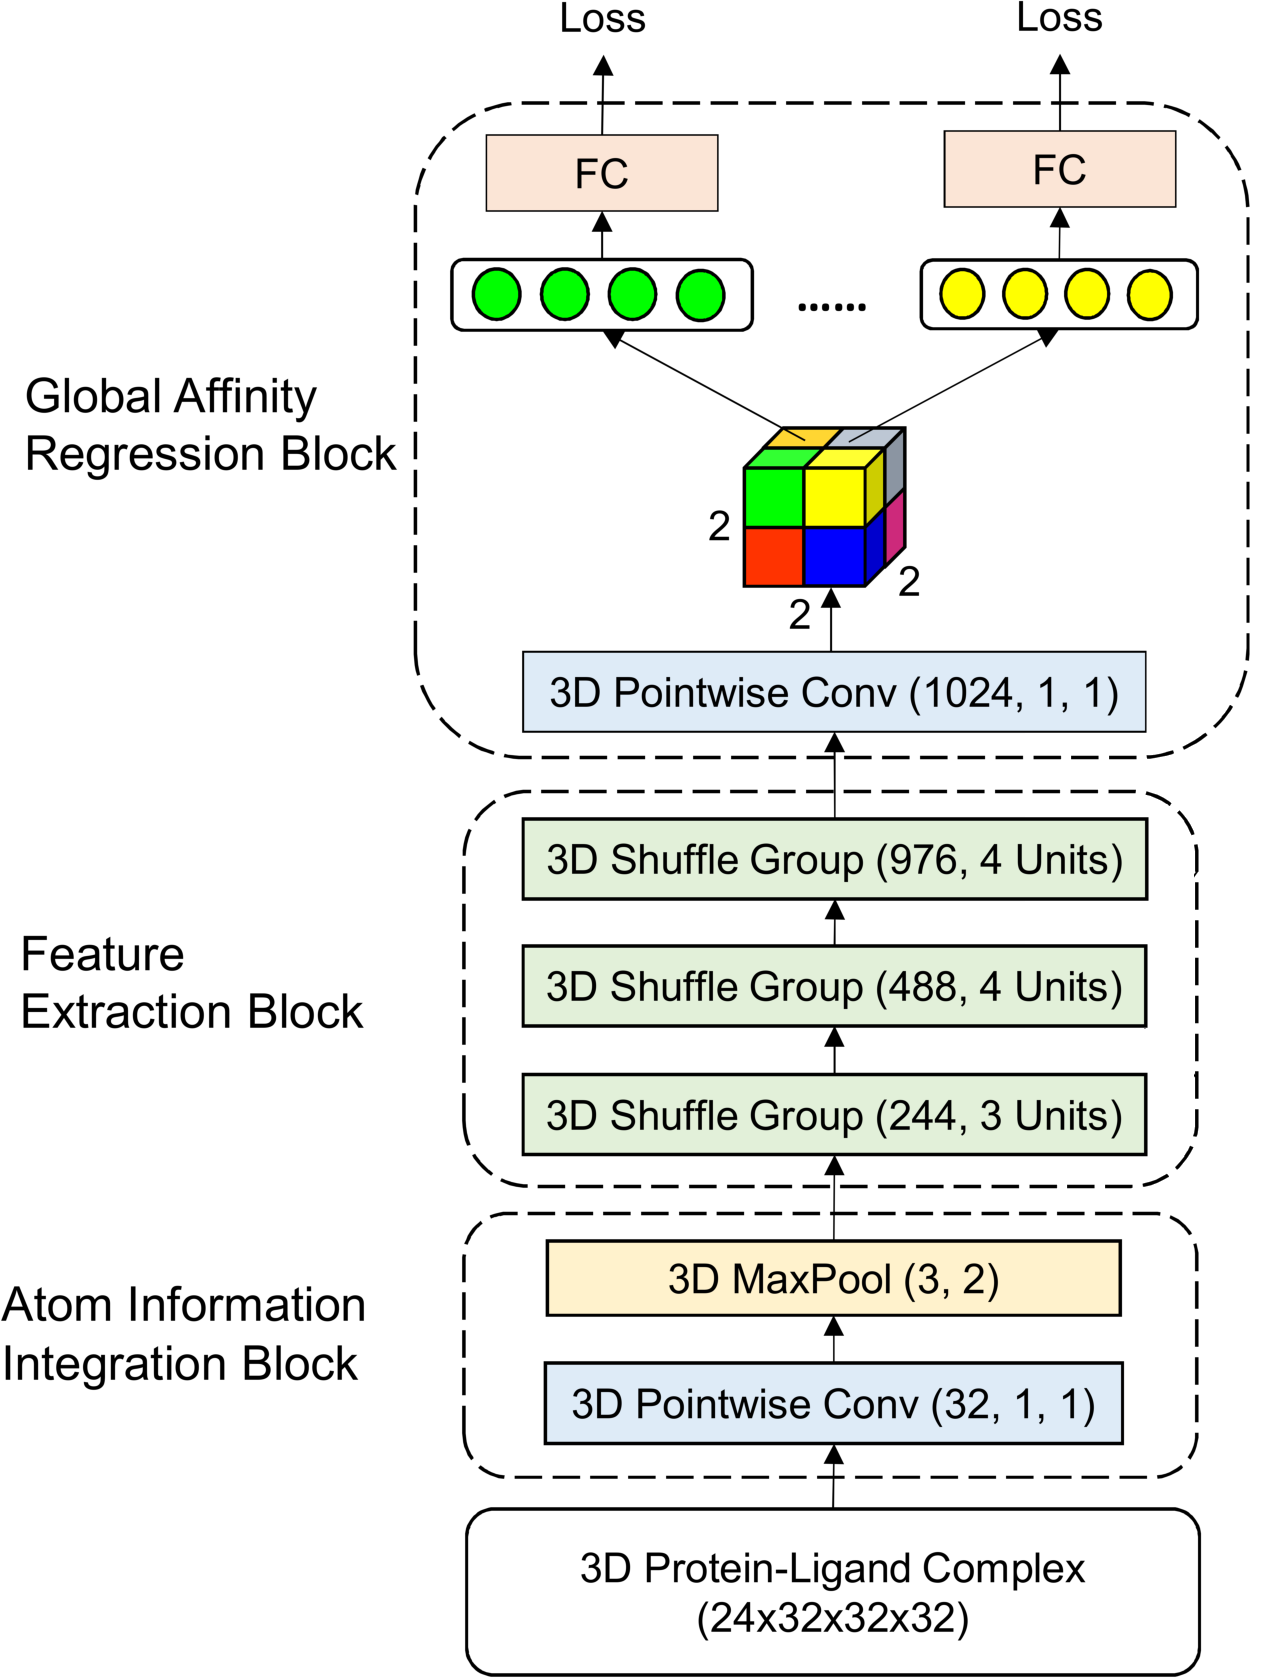
\includegraphics[width=0.55\textwidth]{images/network_left}
        \end{figure}
    \end{columns}
\end{frame}


\subsection{i. Atom information integration block}
\begin{frame}{i. Atom information integration block}
    \textbf{Atomic information across the \sout{24} 
    \textcolor{darkred}{8} channels is aggregate in a 
    pointwise fashion, and the output is then pooled.}
    \begin{enumerate}
        \item $\text{PWConv}(W, h)_{(i, j, k)} = \Sigma_{m}^{24}W_m\cdot 
        h_{(i,j,k,m)}$ is used to map the $8\times32^3$ input to $32^3$.
        \item The max-pooling downsamples the tensor to $16^3$.
    \end{enumerate}
    Semantically, this block processes the input into non-linear function of the linear combination of the various channels (interaction types), parsimoniously.
    \begin{figure}
        \centering
        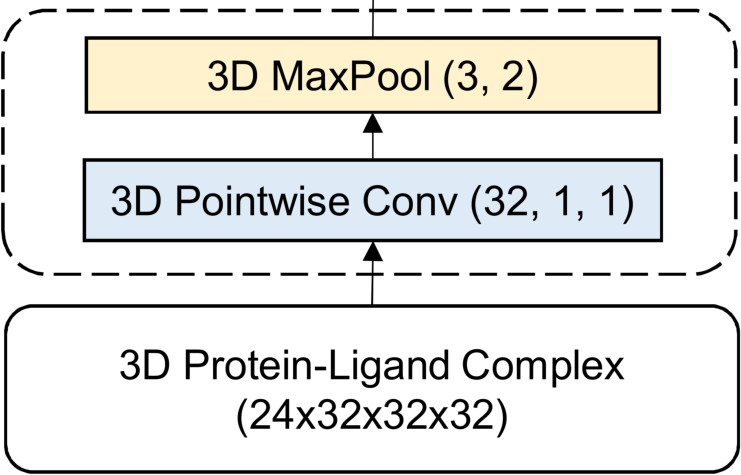
\includegraphics[width=0.3\textwidth]{images/aii_block}
    \end{figure}
\end{frame}


\subsection{ii. Stacked feature extraction block}
\begin{frame}{ii. Stacked feature extraction block}
    \begin{columns}[c]
        \column{.45\textwidth}
        \textbf{Three 3D shuffle groups are stacked, each containing a parsimonious
        combination of pointwise and depthwise convolutions.}
        
        Shuffling, splitting, and then processing only certain channels encourages parsimonious while maintaining performance.
        \newline
        \begin{equation*}
            \text{DWConv}(W, h)_{(i, j, k)} =
        \end{equation*}
        \begin{equation*}
            \Sigma_{s,t,r}^{S, T, R} W_{s,t,r}\odot h_{(i+s,j+t,k+r)}
        \end{equation*}
        \column{.6\textwidth}
        \begin{figure}
            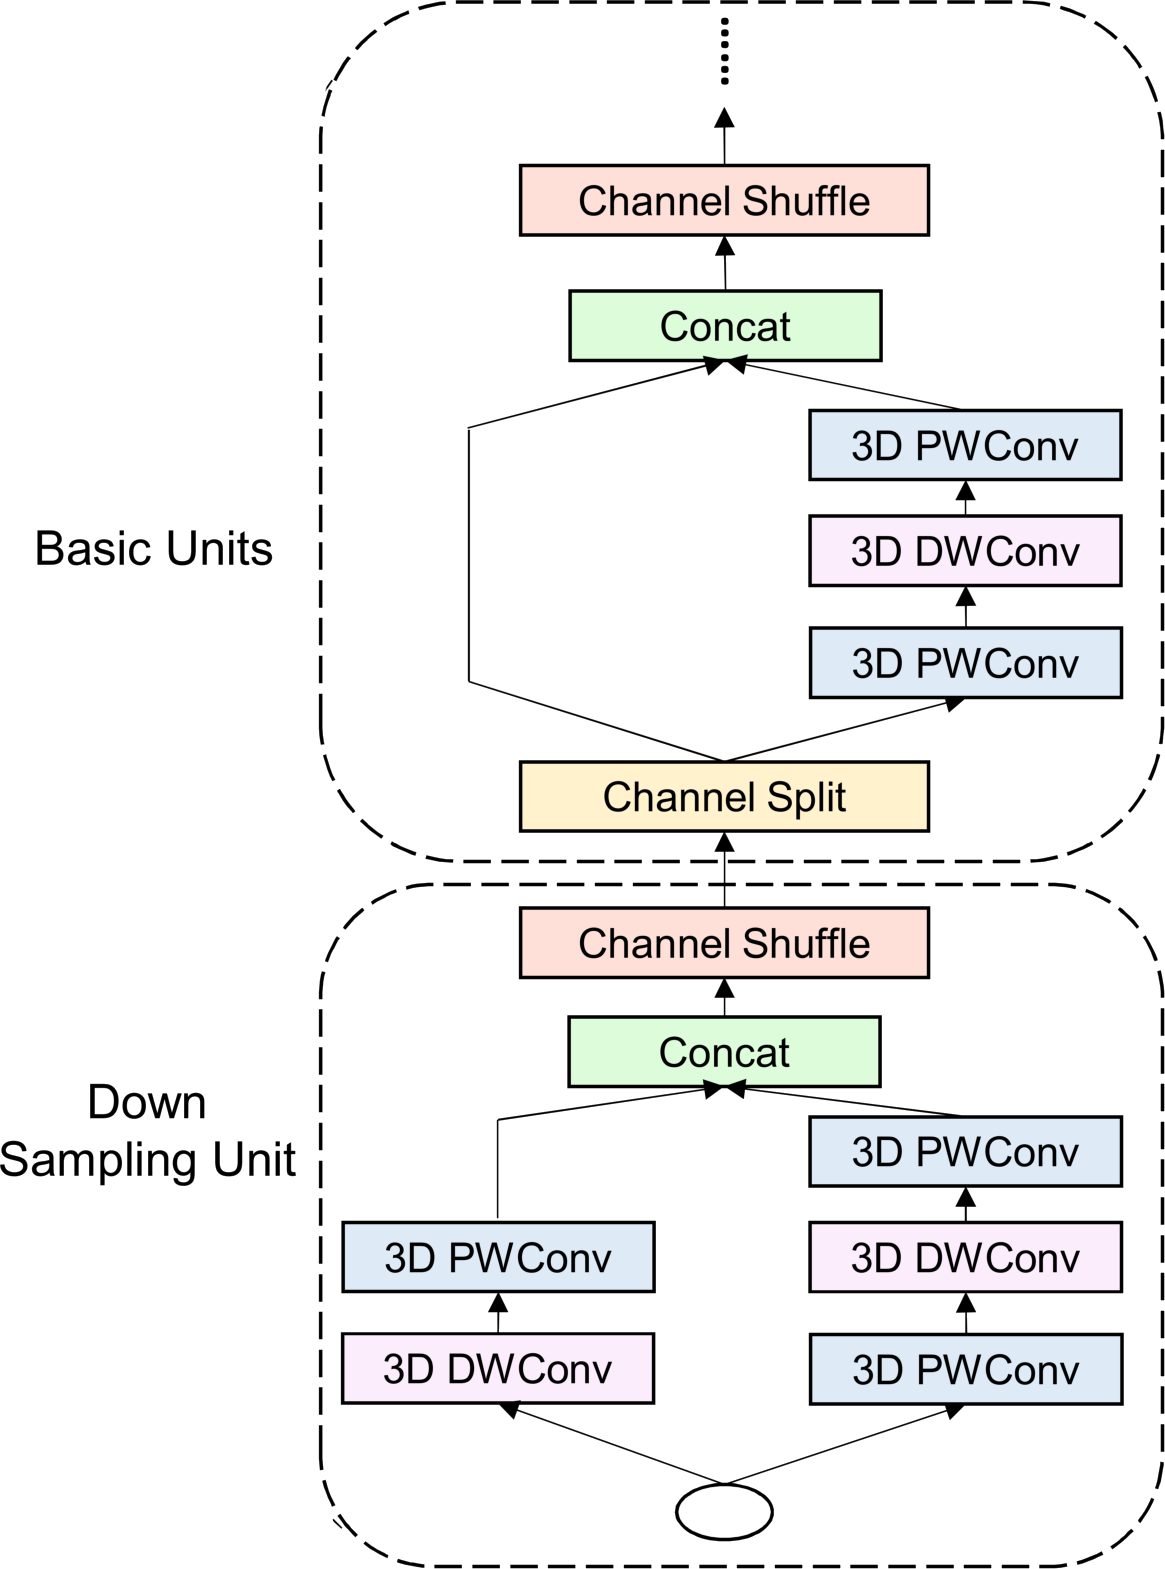
\includegraphics[width=0.55\textwidth]{images/network_right}
        \end{figure}
    \end{columns}
\end{frame}


\subsection{iii. Classification block}
\begin{frame}{iii. Classification Block}
    \begin{columns}[c]
        \column{.45\textwidth}
        \textbf{Previously, an ensemble of eight fully-connected networks}, derived from the eight channels of the output of the second block, are used to create predictions.
        
        Due to overfitting issues, I tried a few simpler approaches, settling on this:
        \begin{enumerate}
            \item A 3D pointwise convolution.
            \item Average pooling.
            \item Flattening into a 976-vector to be passed through a single 976-to-1 fully-connected layer.
        \end{enumerate}
        \column{.6\textwidth}
        \begin{figure}
            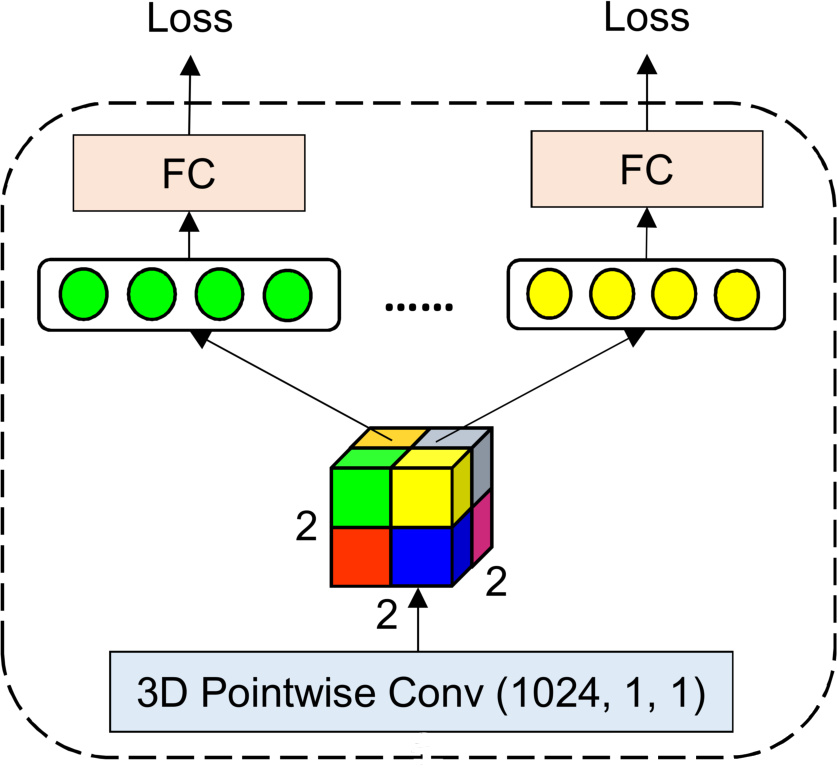
\includegraphics[width=0.7\textwidth]{images/gar_block}\par
            \textit{Previous approach}
        \end{figure}
    \end{columns}
\end{frame}


%------------------------------------------------
\section{Results on DUD-E}
%------------------------------------------------
\subsection{i. Data}
\begin{frame}{Data: a simplified attempt}
    \textcolor{darkgreen}{\textbf{For this initial test, the model had it 
    easy.}}
    \begin{itemize}
        \item \textit{A limited number of proteins:} the model was trained and validated on examples from the \textit{same} 10 proteins.
        \item \textit{A high actives ratio:} the ratio of active ligands to decoys was 1:3, far greater than what occurs naturally.
        \item {No lack of data:} the training set had $\sim13,000$ cocomplexes in total: about double than when this architecture was used for BAP originally.
    \end{itemize}
    \textcolor{darkred}{\textbf{However,}}
    \begin{itemize}
        \item The rasterized 3D cocomplex grid was ``channelized'' into 8 rather than 24 channels, based on the \texttt{MoleculeKit} rather than the \texttt{Arpeggio} package.
    \end{itemize}
\end{frame}


\subsection{ii. Performance}
\begin{frame}{Loss curves}
    \begin{figure}
        \centering
        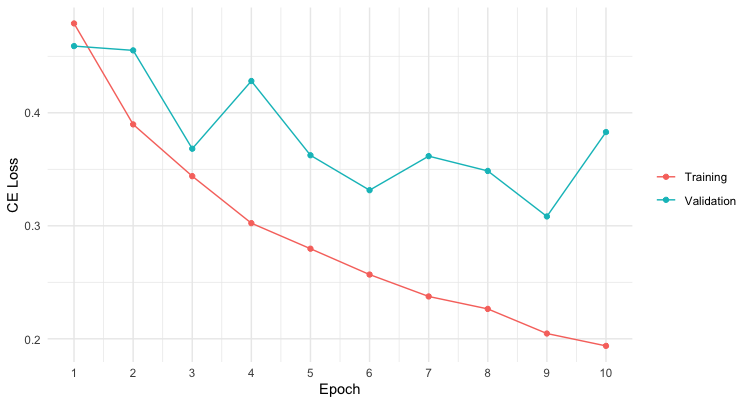
\includegraphics[width=0.85\textwidth]{images/loss_curves}
    \end{figure}
\end{frame}


\begin{frame}{Accuracy curves}
    \begin{figure}
        \centering
        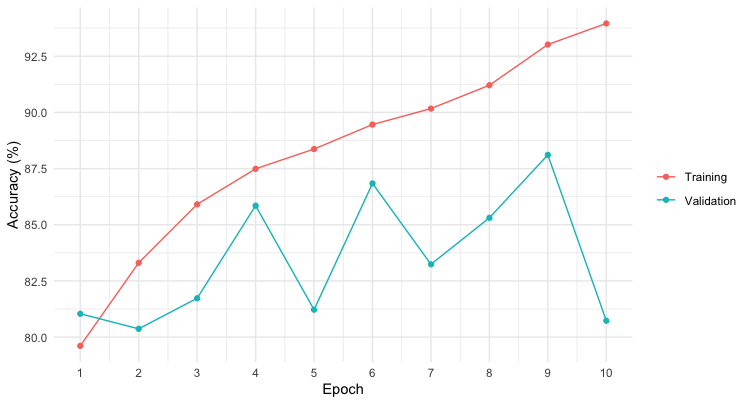
\includegraphics[width=0.85\textwidth]{images/acc_curves}
    \end{figure}
\end{frame}


\begin{frame}{Validation confusion matrix and associated statistics}
    \begin{center}
        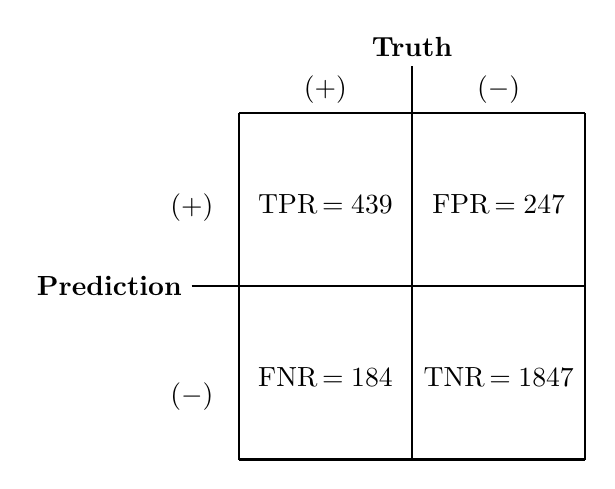
\begin{tikzpicture}[scale=2]
            % Draw Basic Box
            \draw[thick] (0,0) -- (2.2,0);
            \draw[thick] (0,0) -- (0, 2.2);
            \draw[thick] (2.2,2.2) -- (2.2, 0);
            \draw[thick] (2.2,2.2) -- (0, 2.2);
        
            % Draw Box Ticks
            \draw[thick] (-0.3, 1.1) -- (2.2, 1.1);
            \draw[thick] (1.1, 0) -- (1.1, 2.5);
        
            % Box Labels
            % -- left side
            \coordinate[label=left:($+$)] (p1) at (-0.1,1.6);
            \coordinate[label=left:($-$)] (p2) at (-0.1,0.4);
        
            % -- top side
            \coordinate[label=above:($+$)] (p3) at (0.55, 2.2);
            \coordinate[label=above:($-$)] (p4) at (1.65, 2.2);
        
            % -- overall headers
            \coordinate[label=above:\textbf{Truth}] (p5) at (1.1, 2.5);
            \coordinate[label=left:\textbf{Prediction}] (p6) at (-0.3, 1.1);
        

            % Category Values
            \coordinate[label={TPR$\,=439$}] (TPR) at (0.55, 1.50);
            \coordinate[label={FPR$\,=247$}] (FPR) at (1.65, 1.50);
            \coordinate[label={FNR$\,=184$}] (FNR) at (0.55, 0.40);
            \coordinate[label={TNR$\,=1847$}] (TNR) at (1.65, 0.40);
        \end{tikzpicture}
    \end{center}
\end{frame}


\begin{frame}{Evaluation}
    \textcolor{orange}{\textbf{The model has middling performance, and overfits very quickly.}}
    \begin{itemize}
        \item The shuffle groups, while designed to save parameters without 
        increasing the model's bias, are likely too many in number.
        \item The reduced dimensionality of the input due to the fewer channels likely did not help.
        \item The model does not cope well with class imbalance.
    \end{itemize}
    \textcolor{darkgreen}{\textbf{Therefore, some next steps:}}
    \begin{itemize}
        \item Use \texttt{Arpeggio}'s channelization.
        \item Use more data, and weight positive data more highly.
        \item Tune discrete aspects of the network architecture (e.g.: number of layers).
        \item Enable better data processing and optimization using NSCC.
    \end{itemize}
\end{frame}


%------------------------------------------------
\section{}
\begin{frame}{For More Details...}
    \footnotesize{
    DeepAtom:
    \begin{thebibliography}{99}
        \bibitem[Li et al., 2012]{p1} Li, Y., Rezaei, M. A., Li, C., \& Li, X. (2019)
        \newblock DeepAtom: A framework FOR Protein-Ligand binding affinity prediction
        \newblock \emph{IEEE/ACM Transactions on Computational Biology and Bioinformatics}.
    \end{thebibliography}
    \vspace{3mm}
    }
\end{frame}

\end{document}